\documentclass[11pt]{article}
\usepackage[a4paper,margin=25mm]{geometry}
\usepackage{graphicx,amsmath,amssymb,amsthm,booktabs,multirow,float,longtable}
\usepackage[T1]{fontenc}\usepackage{lmodern,microtype}
\usepackage[round,authoryear]{natbib}\usepackage{hyperref,xurl,xr}
\providecommand{\doi}[1]{\url{https://doi.org/#1}}
\input{glyphtounicode}\pdfgentounicode=1
\theoremstyle{plain}
\newtheorem{theorem}{Theorem}\newtheorem{proposition}[theorem]{Proposition}\newtheorem{lemma}[theorem]{Lemma}
\theoremstyle{definition}\newtheorem{remark}{Remark}\newtheorem{example}{Example}
\newcommand{\T}{\mathcal T}\newcommand{\Pp}{\mathbb P}\newcommand{\E}{\mathbb E}\newcommand{\ind}{\mathbf1}
\newif\ifanonymous\ifdefined\blindversion\anonymoustrue\else\anonymousfalse\fi
\newsavebox{\resultsbox}
\raggedbottom\setlength{\emergencystretch}{2em}
\hypersetup{colorlinks=true,linkcolor=black,citecolor=black,urlcolor=blue,pdftitle={Supplementary comparisons and sensitivity analyses},pdfauthor={}}
\externaldocument{main_labels}
\renewcommand{\thesection}{S\arabic{section}}
\renewcommand{\thetable}{S\arabic{table}}
\renewcommand{\thefigure}{S\arabic{figure}}
\renewcommand{\thetheorem}{S\arabic{theorem}}
\title{Online Resource 1\\[4pt]\large Supplementary comparisons and sensitivity analyses\\[5pt]\normalsize Certified degree bounds and shared hubs in correlation spanning trees}
\author{Marek Ga\l{}\k{a}zka and Hanna Wdowicka\\[4pt]\small Computational Statistics\\\small Corresponding author: galazka@amu.edu.pl\\\small Adam Mickiewicz University, Pozna\'n, Poland}
\date{}
\begin{document}\maketitle
This supplement retains the additional calibrations, the full baseline simulation and morphometric grids, the projection timing audit, and the Pearson and Polish-market sensitivity studies. The principal independent-selection validation and ordinal application are reported in the main paper. Complete outcomes for all 20 procedures in the 6600-dataset validation are supplied as machine-readable records; comparisons are within procedures, not a pooled confidence claim across methods.
\section{Additional calibration details}
\subsection{Efficiency and repeated independent matchings}
The disjoint-pair construction exchanges information for an exact conditional test. Randomized incomplete U-statistics offer related statistical/computational trade-offs \citep{chenkato2019}. This cost is explicit at a continuous independence model. For adjacent edges $e=\{v,a\}$ and $f=\{v,b\}$, write $h=H_e-H_f$. Then $\operatorname{Var}(h)=2$. After transforming the three margins to independent uniforms, its first-order projection is
\[
 g(U)=(2U_v-1)\{(2U_a-1)-(2U_b-1)\},\qquad
 \zeta_1=\operatorname{Var}\{g(U)\}=2/9.
\]
The paired estimator has variance $2/N\sim4/n$, while the full order-two U-statistic has asymptotic variance $4\zeta_1/n=8/(9n)$. Their variance ratio is $4.5$, corresponding to about $22\%$ relative efficiency. This calculation describes the continuous independence model; power also depends on the alternative, discordances and the simultaneous-testing family.

We therefore evaluate $R=8$ matchings, the first predetermined and the others independent uniform permutations chosen independently of the measurements. Independent auxiliary tie randomization is used in each matching. Let $p^{(r)}_{ef}$ be its unadjusted one-sided p-value and define
\begin{equation}\label{eq:merge}
 \widetilde p_{ef}=\min\left\{1,\frac{2}{R}\sum_{r=1}^R p^{(r)}_{ef}\right\}.
\end{equation}
For $R=1$ we retain the original p-value. The factor two is the dependence-safe arithmetic-mean merging rule of \citet{vovk2020}. Matchings share observations, so their p-values are dependent.

\begin{proposition}[Finite-sample validity of matching aggregation]\label{prop:merge}
Under the sampling assumptions of Theorem~\ref{thm:finite}, apply Holm to \eqref{eq:merge} over a fixed comparison family. Retain any subset of its rejections and then take transitive closure. The resulting strict orders, and every subsequent degree or rank projection, satisfy the same familywise guarantee $1-\alpha$.
\end{proposition}
\begin{proof}
Conditional on any independently chosen matching, each null p-value is superuniform by Theorem~\ref{thm:finite}. It remains superuniform after averaging over the matching randomization. The arithmetic-mean rule is valid under arbitrary dependence, so every merged null p-value is superuniform. Holm controls any false rejection. Deleting rejections cannot increase this event, and the transitive consequences of true strict orders are true.
\end{proof}
For reproducible closure, the implementation retains only merged rejections consistent with the average paired edge scores. This deletion preserves the guarantee. It does not introduce comparisons that failed Holm. Aggregating p-values reduces dependence on an individual matching, but its power must be measured: the factor two and p-value averaging can be conservative. For comparison, averaging $R$ independently randomized matching \emph{estimators} has variance $\operatorname{Var}(U)+(\operatorname{Var}(V)-\operatorname{Var}(U))/R$, by conditional expectation over matchings. At the independence model its asymptotic variance relative to the full U-statistic is $1+3.5/R$. This estimator calculation alone does not establish an equivalent efficiency for \eqref{eq:merge}.

\subsection{A finite-sample comparator using all observation pairs}
Define $k_e(X_s,X_t)=\operatorname{sgn}(X_{si}-X_{ti})\operatorname{sgn}(X_{sj}-X_{tj})$ and
\[
 \widehat\tau_e={\binom n2}^{-1}\sum_{s<t} k_e(X_s,X_t),\qquad
 \widehat\Delta_{ef}=\widehat\tau_e-\widehat\tau_f.
\]
The difference kernel lies in $[-2,2]$, including ties. Hoeffding's order-two U-statistic inequality \citep{hoeffding1963} gives
\begin{equation}\label{eq:directhoeffding}
 \Pp\{\widehat\Delta_{ef}-\Delta_{ef}\ge t\}
 \le \exp(-Nt^2/8).
\end{equation}
Consequently $p^{U}_{ef}=\exp\{-N(\max\{\widehat\Delta_{ef},0\})^2/8\}$ is superuniform under $\Delta_{ef}\le0$. Holm and the same projections therefore give finite-sample simultaneous inference. To see \eqref{eq:directhoeffding} directly, average the disjoint-pair mean over a uniform random matching conditional on the sample. This conditional average is $\widehat\Delta_{ef}$. Jensen's inequality bounds its exponential moment by that of a mean of $N$ independent kernels of range four; optimizing the usual bounded-variable exponential bound gives \eqref{eq:directhoeffding}. Thus dependence between the $\binom n2$ kernels is respected.

This comparator isolates direct testing from rectangularization while retaining a finite-sample guarantee. Its bounded-range calibration can remain conservative even though its estimator uses all pairs.

\subsection{Local and complete families}
Every fixed comparison family can be used in the exact constructions. We compare all pairs sharing a vertex with all pairs of distinct edges. Their ordered hypothesis counts on a complete graph are $K_{\rm local}=p(p-1)(p-2)$ and $K_{\rm all}=m(m-1)$, with ratio $(p+1)/4$ for $p\ge3$. At $p=52$ these are $132{,}600$ and $1{,}756{,}950$.

Complete comparisons can add nonlocal information relevant to cycle-path constraints, while also increasing the multiplicity penalty and computation. Transitive closure of local orders recovers some nonlocal comparisons, but need not recover all of them. The family ablation measures the resulting trade-off at $p=12$; both families are also evaluated on every cross-sectional application. Local testing remains an explicit computational choice for the larger simulations and the Polish sensitivity study.

\section{A positive-definite example of lost joint information}\label{sec:example}
Consider eight vertices indexed $0,\ldots,7$. In the block $\{0,\ldots,5\}$ let hub correlations be $\rho_{0j}=0.06+t$ for $1\le j\le5$, and leaf correlations $\rho_{ij}=0.04+t$ for $1\le i<j\le5$. Set $\rho_{06}=0.10$, $\rho_{67}=0.15$, all other cross-block correlations to zero, and diagonal entries to one, with $t\in[-0.025,0.025]$.

Every matrix is positive definite: it is symmetric, has positive diagonal and is strictly diagonally dominant; the largest absolute off-diagonal row sum is $0.525$. Every within-block spoke exceeds every within-block leaf edge by $0.02$. The unique optimal tree throughout the curve consists of five spokes, the bridge $06$ and edge $67$. Its degree vector is $(6,1,1,1,1,1,2,1)$, so vertex zero is uniquely first.

Now transform correlations by Fisher's $\operatorname{atanh}$ and subtract the mean across all 28 edges at each $t$. Form the smallest coordinatewise rectangular hull of this centered curve. Global centering removes a common shift across all edges but not a shift restricted to one block. Exact rectangular projection yields degree ranges
\[
 [2,6],\ [1,5]\ (\text{each of five leaves}),\ [2,2],\ [1,1].
\]
The marginal rank construction gives vertex zero $[1,7]$. In contrast, the true local orders along the coupled curve force all seven tree edges and rank $[1,1]$. For a changing edge, the derivative of its centered Fisher weight is bounded below by $1-15/[28(1-0.085^2)]>0$; for a constant edge it is negative. Thus its coordinate extrema occur at the two endpoints. An executable verification is supplied with the code. The uncertainty curve is specified for this deterministic comparison of uncertainty-set shapes. It shows why rectangularization can discard relevant information even when the candidate matrices are positive definite and global centering has already been used.

\section{Matched simulation comparisons}\label{sec:simulation}
\subsection{Models, targets and calibration}
We evaluate eight calibrations on identical data: one-matching exact McNemar--Holm, eight-matching p-value aggregation, evidence aggregation over eight or 64 matchings, direct full-U-statistic Hoeffding--Holm, the full-sample rectangular Hoeffding comparator, Gaussian multiplier contrasts, and Gaussian multiplier edge rectangles. The rectangular methods produce orders over the same fixed family as their direct comparators, and every method passes through the same projections.

For the separated Gaussian model, $X_i=a_i Z+\sqrt{1-a_i^2}\epsilon_i$, with independent standard normals, $a_0=0.99$ and the other loadings equally spaced over $[0.45,0.55]$. The near-tie model uses $a_0=0.8+0.5/\sqrt n$, $a_1=0.8$, with other loadings in $[0.45,0.55]$. The $t_5$ model divides each Gaussian row by an independent $\sqrt{\chi_5^2/5}$. These models have a unique population star centred at zero; their population Kendall weights equal $2\arcsin(\rho)/\pi$.

Gaussian independence and IID uniform coordinates on $\{-1,0,1\}$ evaluate null comparisons and exact ties. Every labelled tree is optimal in these null models, so coverage must include degree ranges $[1,p-1]$ and rank ranges $[1,p]$, rather than the degrees of one tie-broken tree. Two additional Gaussian tree models avoid restricting the comparison to a uniquely dominant star. The chain has parent correlation $0.75$; the two-hub model has bridge correlation $0.5$ and leaf-parent correlation $0.7$, with five leaves attached to each hub at $p=12$. All population tree edges are unique optima, but equal vertex degrees retain their full tied rank ranges.

The 24 cells comprise 7,800 independent datasets. At $p=12$, the three star designs use $n\in\{252,1008,4096\}$ and 200 datasets per cell. At $p=52$, they use $n\in\{252,4096\}$ and 100 per cell. Gaussian null cells at $p=12$ use all three sizes, and at $p=52$ use $n=1008$; the discrete null uses $p=12,n=1008$. Every null cell has 1,000 datasets. Chain and two-hub cells use $p=12,n\in\{1008,4096\}$ and 100 datasets per cell. All tests use $\alpha=0.05$, and multiplier calibration uses 999 draws. Seeds, complete cell definitions and individual outcomes are archived.

We report false-order FWER, simultaneous degree and rank coverage, interval widths, forced edges, possible hubs and unique-hub declarations. Wilson intervals quantify Monte Carlo uncertainty. With 1,000 repetitions, the Monte Carlo standard error at probability $0.05$ is about $0.007$. A single empirical rejection proportion is not interpreted as a proof or disproof of a coverage theorem.

\subsection{Test, projection and family ablations}
For every test we compare marginal rank projection, direct degree-difference projection, degree conservation, and their intersection, using the same screened minor. This isolates computational changes from statistical calibration. For the first 100 datasets in every $p=12$ cell, we also add the cycle-path LP and optimize all ordered degree differences, rather than only anchor differences. Improvements are checked independently with Python arbitrary-precision integers. Empty order relations and a forced single tree have known sharp endpoints, so redundant LP solves are skipped. Path-stage estimates therefore have 100 repetitions per cell and are compared with the corresponding paired subset of the other stages.

The complete-edge comparison family is evaluated on the same first 100 non-null datasets in each $p=12$ cell. All four $p=12$ null cells extend both families to 1,000 datasets. Comparisons of families use matched subsets; differences in reported means do not arise from different simulated samples.

\subsection{A frequency reference from practice}
Bootstrap edge reliability is widely used in correlation networks \citep{tumminello2007,musciotto2018}. On the same $p=12$ separated-star, near-tie and Gaussian-null samples with $n=1008$ and $4096$, we compute 499 ordinary Pearson row-bootstrap trees. Pearson and Kendall have the same population optimal-tree ordering in these Gaussian designs. We record edge selection frequencies and the frequency with which the observed anchor is the unique highest-degree vertex. A threshold of $0.95$ is evaluated as a practical declaration rule, including its false hub and false forced-edge rates. It is a frequency heuristic, not a simultaneous confidence procedure. This reference uses all 200 non-null and all 1,000 null datasets in the six selected cells.

\subsection{Calibration and power results}
Table~\ref{tab:nullnew} reports null FWER for the common minor-plus-joint-rank projection. Exact methods have their finite-sample guarantee; the multiplier methods are evaluated empirically. All cellwise Wilson intervals, simultaneous coverage outcomes and replication records accompany the article.
\begin{table}[htbp]\centering\small
\setlength{\tabcolsep}{4pt}
\caption{False-order FWER at nominal 0.05; 1,000 datasets in each null cell. P: one-matching exact; M8: merged p-values; E8/E64: evidence aggregation over 8/64 matchings; M-C: multiplier contrasts; M-B: multiplier rectangle. Both Hoeffding controls have zero false orders in these cells. All methods use the local family.}\label{tab:nullnew}
\begin{lrbox}{\resultsbox}\begin{tabular}{lrrrrrr}
\toprule
Model, $p$, $n$ & P & M8 & E8 & E64 & M-C & M-B\\
\midrule
Gaussian null, 12, 252 & 0.024 & 0.000 & 0.000 & 0.001 & 0.072 & 0.002\\
Gaussian null, 12, 1008 & 0.029 & 0.000 & 0.000 & 0.000 & 0.062 & 0.003\\
Gaussian null, 12, 4096 & 0.032 & 0.000 & 0.001 & 0.000 & 0.042 & 0.001\\
Discrete null, 12, 1008 & 0.029 & 0.000 & 0.001 & 0.000 & 0.050 & 0.001\\
Gaussian null, 52, 1008 & 0.035 & 0.000 & 0.000 & 0.000 & 0.077 & 0.000\\
\bottomrule\end{tabular}\end{lrbox}\ifdim\wd\resultsbox>\linewidth\resizebox{\linewidth}{!}{\usebox{\resultsbox}}\else\usebox{\resultsbox}\fi\end{table}
The largest one-matching null estimate is 0.035, with an individual Wilson interval [0.025,0.048] (Gaussian null, $p=52$, $n=1008$). This is a cellwise Monte Carlo summary; simultaneous calibration is established by the exact-test argument.
\begin{table}[htbp]\centering\small
\setlength{\tabcolsep}{4pt}
\caption{Probability of declaring the true unique hub using the same minor and joint-rank projection. Local comparisons; 200 repetitions for the displayed $p=12$ star cells and 100 for $p=52$. Both Hoeffding controls declare no unique hub in these star cells; full results are archived. Path projection is evaluated separately on paired subsets.}\label{tab:powernew}
\begin{lrbox}{\resultsbox}\begin{tabular}{lrrrrrr}
\toprule
Model, $p$, $n$ & P & M8 & E8 & E64 & M-C & M-B\\
\midrule
Gaussian star, 12, 1008 & 0.000 & 0.000 & 0.000 & 0.000 & 1.000 & 0.900\\
Gaussian star, 12, 4096 & 1.000 & 0.990 & 1.000 & 1.000 & 1.000 & 1.000\\
$t_5$ star, 12, 1008 & 0.000 & 0.000 & 0.000 & 0.000 & 1.000 & 0.195\\
$t_5$ star, 12, 4096 & 1.000 & 1.000 & 1.000 & 1.000 & 1.000 & 1.000\\
Gaussian star, 52, 4096 & 0.670 & 0.000 & 1.000 & 1.000 & 1.000 & 1.000\\
$t_5$ star, 52, 4096 & 0.720 & 0.000 & 1.000 & 1.000 & 1.000 & 1.000\\
Near-tie star, 12, 4096 & 0.000 & 0.000 & 0.000 & 0.000 & 0.000 & 0.000\\
Near-tie star, 52, 4096 & 0.000 & 0.000 & 0.000 & 0.000 & 0.000 & 0.000\\
\bottomrule\end{tabular}\end{lrbox}\ifdim\wd\resultsbox>\linewidth\resizebox{\linewidth}{!}{\usebox{\resultsbox}}\else\usebox{\resultsbox}\fi\end{table}
Power is interpreted jointly with FWER. The multiplier contrast procedure exceeds nominal error in some IID null cells; higher declaration rates in those regimes do not establish valid superiority. The exact evidence methods provide a comparison whose error guarantee does not rely on the Gaussian approximation.
Figure~\ref{fig:powernew} compares the full sample-size grids. The merged rule is assessed as an exact alternative, rather than assumed to recover U-statistic efficiency. The bounded-range U-statistic comparator shows whether using all pairs alone is sufficient; the matched multiplier rectangle and contrast procedures isolate the effect of shared-edge covariance and direct calibration.
\begin{figure}[htbp]\centering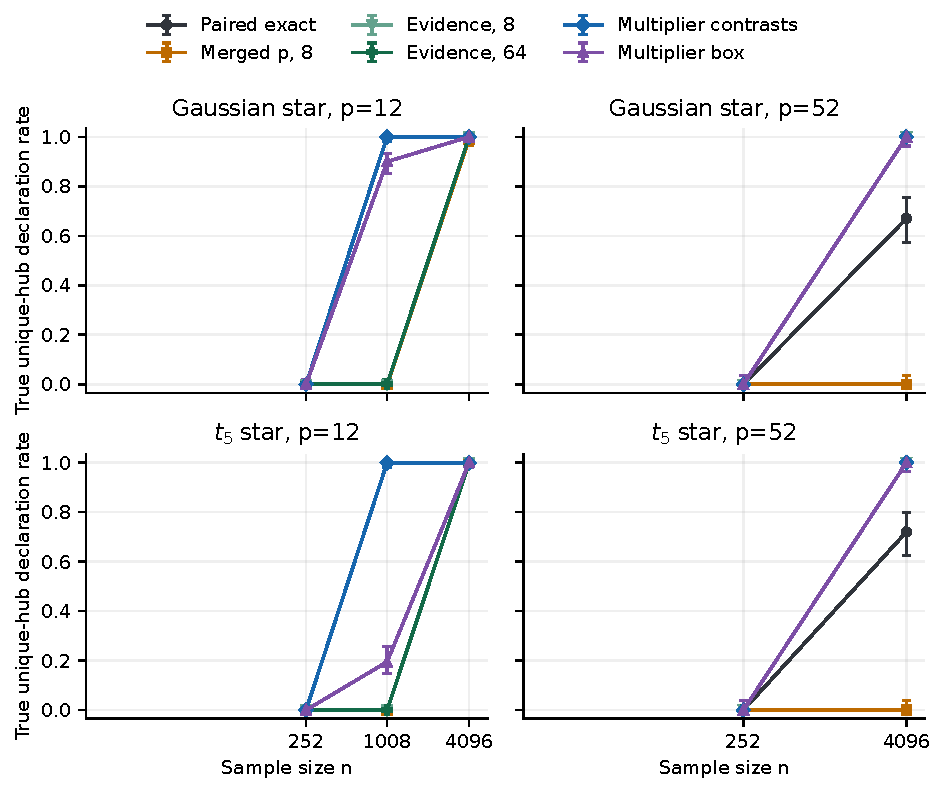
\includegraphics[width=\textwidth]{Fig_comparative.pdf}
\caption{Unique-hub declarations under the common joint projection. Curves use matched data; intervals are individual 95\% Wilson Monte Carlo intervals. All specified sample sizes and both separated distributions are shown.}\label{fig:powernew}\end{figure}
\subsection{Projection ablation}
\begin{table}[htbp]\centering\small
\setlength{\tabcolsep}{4pt}
\caption{Paired projection ablation at $p=12,n=1008$, using the same first 100 datasets per cell. Degree widths compare the minor with path LP. Rank widths compare marginal, joint pair/conservation and path projection. Complete results for all eight tests and sizes are archived. Width is upper minus lower endpoint.}\label{tab:ablation}
\begin{lrbox}{\resultsbox}\begin{tabular}{llrrrrr}
\toprule
Model & Test & $W_d$ minor & $W_d$ path & $W_r$ marg. & $W_r$ joint & $W_r$ path\\
\midrule
Gaussian star & P & 8.94 & 8.40 & 11.00 & 11.00 & 11.00\\
Gaussian star & E64 & 9.02 & 8.33 & 11.00 & 11.00 & 11.00\\
Gaussian star & M-C & 0.00 & 0.00 & 9.17 & 9.17 & 9.17\\
Near-tie star & P & 9.92 & 9.45 & 11.00 & 11.00 & 11.00\\
Near-tie star & E64 & 9.99 & 9.51 & 11.00 & 11.00 & 11.00\\
Near-tie star & M-C & 3.93 & 3.54 & 11.00 & 10.90 & 10.81\\
Chain & P & 8.00 & 4.58 & 11.00 & 11.00 & 11.00\\
Chain & E64 & 6.477 & 3.968 & 11.00 & 10.99 & 10.99\\
Chain & M-C & 0.00 & 0.00 & 7.67 & 7.67 & 7.67\\
Two hubs & P & 8.43 & 6.66 & 11.00 & 10.96 & 10.96\\
Two hubs & E64 & 5.82 & 5.11 & 10.98 & 10.54 & 10.54\\
Two hubs & M-C & 0.58 & 0.58 & 7.67 & 7.67 & 7.67\\
\bottomrule\end{tabular}\end{lrbox}\ifdim\wd\resultsbox>\linewidth\resizebox{\linewidth}{!}{\usebox{\resultsbox}}\else\usebox{\resultsbox}\fi\end{table}
Table~\ref{tab:ablation} locates the path-projection gain mainly in degree precision. For one-matching inference, Gaussian-star mean degree width decreases from 8.94 to 8.40; in the chain it decreases from 8.00 to 4.58. The corresponding E64 chain widths decrease from 6.477 to 3.968. Most exact rank widths remain approximately 11, the full-range width at $p=12$. In the near-tie multiplier example, the path stage decreases mean rank width only from 10.90 to 10.81. Thus these $n=1008$ simulations demonstrate useful degree restrictions but little additional rank resolution: tighter degree bounds need not establish a positive degree difference between two vertices.

Population degree ties also impose an irreducible rank width. Even with the exact Gaussian-star tree known, its eleven leaves occupy ranks 2--12 under the tie-inclusive target, giving mean rank width $110/12=9.17$. For the chain and two-hub trees, the corresponding mean is $92/12=7.67$. The displayed multiplier results at these widths therefore retain the required tied ranks. Degree-conservation and direct-pair rank outputs are archived separately from the path stage.

Across all sample sizes and methods in the $p=12$ simulation path stage{,} the local family accounts for 950{,}820 LP objectives and 375{,}946 independently verified improving rational certificates. The complete family adds 913{,}068 objectives and 273{,}901 certificates. The totals across both families are therefore 1{,}863{,}888 LP objectives and 649{,}847 certificates. These totals include all evaluated path-stage cells{,} rather than only the subset displayed in Table~\ref{tab:ablation}.
\subsection{Comparison-family ablation}
\begin{table}[htbp]\centering\small
\setlength{\tabcolsep}{4pt}
\caption{Matched local/complete family ablation at $p=12,n=4096$, 100 datasets per cell. Closed-order counts use the same $m(m-1)$ potential ordered pairs in either family. More tested comparisons also incur a larger multiplicity penalty.}\label{tab:family}
\begin{lrbox}{\resultsbox}\begin{tabular}{llrrrrrr}
\toprule
Model & Test & Orders L & Orders A & $W_d$ L & $W_d$ A & $W_r$ L & $W_r$ A\\
\midrule
Gaussian star & P & 113.0 & 530.7 & 0.14 & 0.25 & 9.17 & 9.17\\
Gaussian star & E64 & 110.8 & 579.0 & 0.00 & 0.00 & 9.17 & 9.17\\
Gaussian star & M-C & 214.4 & 643.0 & 0.00 & 0.00 & 9.17 & 9.17\\
$t_5$ star & P & 112.0 & 527.8 & 0.17 & 0.31 & 9.17 & 9.17\\
$t_5$ star & E64 & 110.5 & 573.7 & 0.00 & 0.00 & 9.17 & 9.17\\
$t_5$ star & M-C & 193.3 & 629.0 & 0.00 & 0.00 & 9.17 & 9.17\\
Near-tie star & P & 137.3 & 331.6 & 6.40 & 7.20 & 11.00 & 11.00\\
Near-tie star & E64 & 170.8 & 393.1 & 5.53 & 6.54 & 10.99 & 11.00\\
Near-tie star & M-C & 331.1 & 969.4 & 1.66 & 1.67 & 10.16 & 10.17\\
Chain & P & 850.2 & 1338.6 & 0.14 & 0.00 & 7.98 & 7.67\\
Chain & E64 & 923.0 & 1396.0 & 0.00 & 0.00 & 7.67 & 7.67\\
Chain & M-C & 1374.2 & 1766.2 & 0.00 & 0.00 & 7.67 & 7.67\\
Two hubs & P & 624.1 & 1117.3 & 0.99 & 0.38 & 7.67 & 7.67\\
Two hubs & E64 & 659.5 & 1157.1 & 0.97 & 0.02 & 7.67 & 7.67\\
Two hubs & M-C & 725.3 & 1538.1 & 0.00 & 0.00 & 7.67 & 7.67\\
\bottomrule\end{tabular}\end{lrbox}\ifdim\wd\resultsbox>\linewidth\resizebox{\linewidth}{!}{\usebox{\resultsbox}}\else\usebox{\resultsbox}\fi\end{table}
Table~\ref{tab:family} shows a model-dependent trade-off. For one-matching inference in the Gaussian star, complete comparisons increase mean degree width from 0.14 to 0.25 despite increasing the closed-order count from 113.0 to 530.7. In the near-tie E64 example, width increases from 5.53 to 6.54. Conversely, complete comparisons improve the one-matching chain width from 0.14 to 0.00 and the two-hub width from 0.99 to 0.38; for E64 in the two-hub model they reduce it from 0.97 to 0.02.

The procedures recalibrate their tested families, so their rejected-order relations need not be nested. At $p=12$, the local and complete families contain 1,320 and 4,290 ordered hypotheses. For the Holm methods, the first threshold decreases from $0.05/1320$ to $0.05/4290$; multiplier contrasts also recalibrate a larger maximum. This can remove weak local comparisons important to screening incident hub edges, while adding many nonlocal orders. The number of certified orders alone therefore does not determine degree resolution. Holding one valid relation fixed and adding further valid comparisons can only tighten exact bounds over the resulting outer family; changing the calibrated relation is a different comparison. Complete testing is useful when its additional tree restrictions outweigh its multiplicity cost, as in the chain and two-hub examples.
\subsection{Frequency-reference results}
\begin{table}[H]\centering\small
\setlength{\tabcolsep}{4pt}
\caption{Practical row-bootstrap frequency rule on matched Gaussian samples, $p=12$, 499 draws. Hub declarations require unique-hub frequency at least 0.95; edge declarations require selection frequency at least 0.95. False edge declarations are familywise events. Frequencies have no general confidence guarantee.}\label{tab:frequency}
\begin{lrbox}{\resultsbox}\begin{tabular}{lrrrrr}
\toprule
Model & $n$ & $R$ & True hub & False hub & False edge\\
\midrule
Gaussian star & 1008 & 200 & 1.000 & 0.000 & 0.000\\
Gaussian star & 4096 & 200 & 1.000 & 0.000 & 0.000\\
Gaussian null & 1008 & 1000 & -- & 0.000 & 0.043\\
Gaussian null & 4096 & 1000 & -- & 0.000 & 0.049\\
Near-tie star & 1008 & 200 & 0.020 & 0.000 & 0.220\\
Near-tie star & 4096 & 200 & 0.060 & 0.000 & 0.225\\
\bottomrule\end{tabular}\end{lrbox}\ifdim\wd\resultsbox>\linewidth\resizebox{\linewidth}{!}{\usebox{\resultsbox}}\else\usebox{\resultsbox}\fi\end{table}
The frequency reference targets estimated-tree stability. Under the Gaussian null every edge can occur in an optimal population tree, but none is necessary and no vertex is a population unique hub. A high-frequency edge declaration is therefore counted as false necessity in that setting. This definition avoids interpreting frequent selection as a simultaneous population certificate.

\subsection{Decisions gained on the same simulated samples}\label{sec:decision-simulation}
An interval-width reduction is useful for a given question only if it changes the answer or the degree range relevant to that question. We therefore separately count fixed degrees, exclusions from hub status and unique-hub declarations. Table~\ref{tab:decision-simulation} uses the same first 100 samples for both projections and retains every non-null $p=12$ model at $n=1008$ and $4096$. The archived audit includes all 17 $p=12$ cells, both families and all eight calibrations, giving 27,200 paired method--family--dataset comparisons. These are repeated analyses of the original datasets, not new independent samples.


\begin{table}[H]\centering\small
\setlength{\tabcolsep}{4pt}
\caption{Paired E64 decision yield, local family, $p=12$. Fixed degrees and hub exclusions are mean counts per dataset before (M: minor with pair/conservation ranks) and after full path projection (F). The last column counts datasets gaining a fixed degree, a hub exclusion or a unique-hub declaration. Each row contains the same 100 samples in both stages.}\label{tab:decision-simulation}
\begin{lrbox}{\resultsbox}\begin{tabular}{llrrrrr}
\toprule
Model & $n$ & Fixed M & Fixed F & Excluded M & Excluded F & Any gain\\
\midrule
Gaussian star & 1008 & 0.00 & 0.00 & 0.00 & 0.00 & 0/100\\
Gaussian star & 4096 & 12.00 & 12.00 & 11.00 & 11.00 & 0/100\\
$t_5$ star & 1008 & 0.00 & 0.00 & 0.00 & 0.00 & 0/100\\
$t_5$ star & 4096 & 12.00 & 12.00 & 11.00 & 11.00 & 0/100\\
Near tie & 1008 & 0.00 & 0.00 & 0.00 & 0.00 & 0/100\\
Near tie & 4096 & 0.06 & 0.21 & 0.06 & 0.21 & 13/100\\
Chain & 1008 & 0.00 & 0.00 & 0.00 & 0.00 & 0/100\\
Chain & 4096 & 12.00 & 12.00 & 2.00 & 2.00 & 0/100\\
Two hubs & 1008 & 0.00 & 0.00 & 0.12 & 0.16 & 1/100\\
Two hubs & 4096 & 0.40 & 0.40 & 10.00 & 10.00 & 0/100\\
\bottomrule\end{tabular}\end{lrbox}\ifdim\wd\resultsbox>\linewidth\resizebox{\linewidth}{!}{\usebox{\resultsbox}}\else\usebox{\resultsbox}\fi\end{table}


At $n=1008$, neither exact star experiment yields a fixed degree or a hub exclusion, even after full projection. For the chain, degree width falls from $6.48$ to $3.97$ without changing these decisions. For near ties at $n=4096$, projection produces a new decision in 13 of 100 samples: the mean number of fixed degrees and excluded hubs both increase from $0.06$ to $0.21$, but no unique hub is identified. The two-hub model at $n=1008$ gains exclusions in one of 100 samples. At $n=4096$, separated-star hubs are already identified by the minor stage; the additional LP work does not create that success. Thus the exact method's larger-sample power comes primarily from calibrated edge evidence, while projection has selective value for partial decisions. Full cellwise counts and original coverage results accompany the article.


\section{Cross-sectional morphometric applications}\label{sec:crosssection}
\subsection{Recorded measurements and sampling scope}
The morphometric application uses all 4,177 specimens in the UCI Abalone dataset \citep{abalone1994}. Vertices are its eight numerical measurements: length, diameter, height, whole weight, shucked weight, viscera weight, shell weight and ring count. The recorded sex/status field defines three additional reported strata (female, male and infant). Original supplied measurements are retained, including zero heights and tied ring counts; no outlier removal, imputation or residual fitting is performed. The supplied complete-case dataset has no identical full rows. One independently generated permutation fixes the observation ordering before disjoint pairing.

The sampling model treats specimens as independent observations from one common distribution within each analysed population. This is a working model for cross-sectional measurements. The repository does not provide specimen identifiers, sampling clusters or acquisition batches sufficient to establish independence from the files alone. Pooled and sex-stratified results are all reported, and heterogeneity across strata is examined explicitly. The finite-sample guarantee is conditional on this IID sampling model. The nominal error level applies within one stated method and comparison family, not jointly across all reported analyses.

As a secondary computational stress study, we apply all methods to the 16 image-derived features of UCI Dry Bean, pooled and separately for all seven varieties \citep{drybean2020}. This file contains 68 repeated full rows and several mechanically related shape measurements. We retain them and report ties and degenerate contrasts. These cases assess projection and tie handling; their sampling design is insufficiently documented for an unconditional population confidence interpretation. Morphometric correlation trees describe association among measurements, including measurement identities, rather than causal or conditional-independence networks.

\subsection{Exact, merged and multiplier outputs}
All eight methods and both comparison families are applied to all 12 datasets. Every projection includes all degree and ordered degree-difference LP objectives, with independent rational verification of improvements. Ordinary row-bootstrap Kendall trees, using 499 resamples and the complete tau-a statistic, supply edge frequencies and unique-hub frequencies on the same data. These frequencies remain separate from the exact confidence statements. Original datasets are redistributed under their CC BY 4.0 licences, with source citations and unchanged-file hashes.

\begin{table}[htbp]\centering\small
\setlength{\tabcolsep}{4pt}
\caption{Primary Abalone application, $n=4177,p=8$, local family. P, M8, E8, E64, U-H and H-box have finite-sample guarantees under the stated IID sampling model; M-C and M-B use asymptotic multiplier calibration. Bounds in this table are from the same full degree-pair path-LP projection. Exact enumeration (main text, Section~\ref{sec:sharp}) further sharpens several E64 endpoints, including the Height degree from $[1,3]$ to $[1,2]$, and raises the number of hub exclusions from four to five.}\label{tab:abalone}
\begin{lrbox}{\resultsbox}\begin{tabular}{lrrrrrrr}
\toprule
Test & Orders & Forced & Fixed degrees & Hubs & $W_d$ minor & $W_d$ path & $W_r$\\
\midrule
P & 104 & 0 & 1 & 0 & 3.250 & 2.625 & 6.750\\
M8 & 89 & 0 & 0 & 0 & 4.250 & 3.250 & 7.000\\
E8 & 109 & 3 & 1 & 0 & 2.125 & 1.875 & 6.500\\
E64 & 111 & 3 & 2 & 0 & 1.875 & 1.375 & 5.625\\
U-H & 42 & 0 & 0 & 0 & 6.000 & 5.500 & 7.000\\
H-box & 45 & 0 & 0 & 0 & 6.000 & 5.250 & 7.000\\
M-C & 152 & 6 & 6 & 1 & 0.250 & 0.250 & 3.250\\
M-B & 125 & 4 & 3 & 1 & 0.875 & 0.750 & 4.875\\
\bottomrule\end{tabular}\end{lrbox}\ifdim\wd\resultsbox>\linewidth\resizebox{\linewidth}{!}{\usebox{\resultsbox}}\else\usebox{\resultsbox}\fi\end{table}
For the single-matching exact reference, path projection reduces mean degree width from 3.250 to 2.625 (19.2\%). Ring count has degree [1,1] and rank [3,8], excluding hub status under the stated model. Whole weight appears as the unique sample hub in all 499 ordinary Kendall bootstrap trees, but its one-matching exact rank remains [1,8]. The multiplier-contrast projection instead gives whole-weight degree [4,4] and rank [1,1]. This nominal bootstrap declaration and the exact confidence output are reported separately.
The estimated Pearson and Kendall Abalone trees share 5 of seven edges. Both weight definitions and all edge frequencies are archived. Their agreement in this dataset does not make the population targets interchangeable outside models with a common monotone correlation ordering. Pooled and sex-stratified results, every complete-family comparison, and all Dry Bean stress outputs are supplied without selecting favorable strata.
The exact E64 construction gives whole-weight degree [3,5] and rank [1,3], excluding 4 of the eight vertices from hub status. Its mean degree width is 1.375, 47.6\% below the single-matching exact result after the same projection. It retains a finite-sample guarantee under the same sampling model; unique-hub identification and a top-three rank restriction are distinct conclusions.
\begin{figure}[!ht]\centering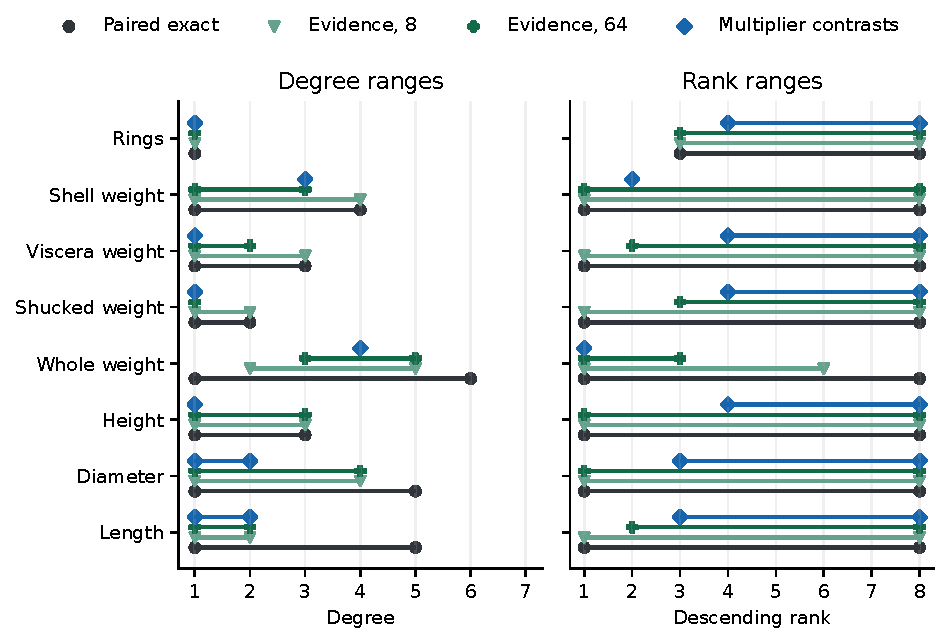
\includegraphics[width=\textwidth]{Fig_cross_section.pdf}
\caption{Degree and rank ranges for eight Abalone measurements under the four displayed calibrations, after identical path projection. P, E8 and E64 have finite-sample guarantees under the stated IID model; M-C has asymptotic multiplier calibration. Population degree ties retain their full rank ranges.}\label{fig:cross}\end{figure}

\subsection{Which conclusions change after projection?}\label{sec:decision-application}
The primary question is which measurements can be certified as leaves, excluded from hub status, or placed within the top three. These are statements about the marginal association tree; leaf status alone does not justify removing a measurement from a predictive model. Table~\ref{tab:decision-abalone} separates the gain from replacing one matching by E64 from the gain due to subsequent optimization.


\begin{table}[H]\centering\small
\setlength{\tabcolsep}{4pt}
\caption{Abalone pooled: concrete conclusions under the IID working model and a separately chosen calibration. All rows use local edge comparisons. Fixed and excluded denote counts among eight measurements. The last two columns concern whole weight. P is one-matching exact McNemar--Holm. The Full LP rows use path projection. Exact enumeration (main text, Section~\ref{sec:sharp}) further improves E64 Height degree from $[1,3]$ to $[1,2]$ and raises hub exclusions from four to five.}\label{tab:decision-abalone}
\begin{lrbox}{\resultsbox}\begin{tabular}{llrrrr}
\toprule
Test & Projection & Fixed & Excluded & Degree & Rank\\
\midrule
P & Full LP & 1 & 1 & [1,6] & [1,8]\\
E64 & Minor & 1 & 2 & [2,5] & [1,6]\\
E64 & Degree LP & 2 & 4 & [3,5] & [1,3]\\
E64 & Full LP & 2 & 4 & [3,5] & [1,3]\\
\bottomrule\end{tabular}\end{lrbox}\ifdim\wd\resultsbox>\linewidth\resizebox{\linewidth}{!}{\usebox{\resultsbox}}\else\usebox{\resultsbox}\fi\end{table}


With E64 fixed, the minor stage excludes length and shucked weight from hub status. Degree-only path projection additionally excludes viscera weight and ring count, certifies ring count as a leaf, and raises the lower degree of whole weight from two to three. Together with degree conservation, these statements place whole weight within the top three. It is certified to have strictly greater degree than length, shucked weight, viscera weight and ring count in every population-optimal tree. The extra 56 ordered-pair LP objectives change none of the reported degree or rank endpoints. The top-three statement has a simple structural explanation. The eight degrees sum to 14. If whole weight and three competitors each had degree at least three, these four vertices plus the four remaining positive degrees would sum to at least 16. At most two competitors can therefore match or exceed whole weight. The inferential conclusion is four excluded hubs and a top-three restriction, with the identity of a unique population hub still unresolved.

Table~\ref{tab:decision-populations} reports the entire E64 local-family measurement grid, including cases with no new decision. At $n=1307$ and $1528$, degree LP certifies ring count as a leaf in the female and male Abalone strata, respectively; neither minor projection resolves those degrees. In the infant stratum, shucked weight is already a certified leaf before LP. The corresponding guarantees require an IID model separately within each analysed population. The comparisons across populations, methods and families are descriptive and have no joint 95\% coverage statement.


\begin{table}[H]\centering\small
\setlength{\tabcolsep}{4pt}
\caption{All 12 measurement populations: E64 local-family decision counts, minor $\to$ degree-only LP. Full ordered-pair projection gives the same rank endpoints as degree-only LP in every row. Dry Bean remains a computational stress study because the sampling design and repeated rows limit a population interpretation.}\label{tab:decision-populations}
\begin{lrbox}{\resultsbox}\begin{tabular}{lrrrrr}
\toprule
Population & $n$ & $p$ & Fixed & Excluded & Top three\\
\midrule
Abalone pooled & 4177 & 8 & 1 $\to$ 2 & 2 $\to$ 4 & 0 $\to$ 1\\
Abalone F & 1307 & 8 & 0 $\to$ 1 & 0 $\to$ 1 & 0 $\to$ 0\\
Abalone I & 1342 & 8 & 1 $\to$ 1 & 1 $\to$ 1 & 0 $\to$ 0\\
Abalone M & 1528 & 8 & 0 $\to$ 1 & 0 $\to$ 1 & 0 $\to$ 0\\
Bean Barbunya & 1322 & 16 & 0 $\to$ 0 & 0 $\to$ 0 & 0 $\to$ 0\\
Bean Bombay & 522 & 16 & 0 $\to$ 0 & 0 $\to$ 0 & 0 $\to$ 0\\
Bean Cali & 1630 & 16 & 0 $\to$ 0 & 0 $\to$ 0 & 0 $\to$ 0\\
Bean Dermason & 3546 & 16 & 0 $\to$ 0 & 0 $\to$ 0 & 0 $\to$ 0\\
Bean Horoz & 1928 & 16 & 0 $\to$ 0 & 0 $\to$ 0 & 0 $\to$ 0\\
Bean Seker & 2027 & 16 & 0 $\to$ 0 & 0 $\to$ 0 & 0 $\to$ 0\\
Bean Sira & 2636 & 16 & 0 $\to$ 0 & 0 $\to$ 0 & 0 $\to$ 0\\
Bean Pooled & 13611 & 16 & 0 $\to$ 0 & 0 $\to$ 0 & 0 $\to$ 0\\
\bottomrule\end{tabular}\end{lrbox}\ifdim\wd\resultsbox>\linewidth\resizebox{\linewidth}{!}{\usebox{\resultsbox}}\else\usebox{\resultsbox}\fi\end{table}


Across all 192 original method--family--population analyses, degree-only LP adds at least one of the stated decisions in 32 analyses. Full pair projection gives exactly the same rank endpoints in 188 of 192 analyses. Its remaining benefit is six additional hub exclusions across four analyses: female Abalone with multiplier rectangles and male Abalone with P, each under both comparison families. These four analyses concern two populations and are not independent confirmations. No stage produces a new unique-hub declaration on the measurement grid. Dry Bean's E64 degree widths narrow, but no leaf, hub exclusion or top-three restriction is certified, even in the pooled sample of 13,611 records. This distinguishes a narrower numerical bound from a new substantive conclusion.


\section{Computation matched to the inferential question}\label{sec:cost}
The decision-first workflow uses a fixed calibration and comparison family, then adds optimization only for the desired output. We benchmark one-matching P and E64 on all 12 measurement populations and the first replication of each of the 13 $p=12$ simulation cells with $n\ge1008$: 50 cases in total. This sample rule is independent of benchmark outcomes. Each case and stage runs in a fresh process, with one untimed warm-up and three timed repetitions, serial execution, one pinned CPU, and one BLAS/OpenMP/HiGHS thread. Interpreter startup and data loading are excluded. Projection timings include the minor construction, LP work and independent rational-certificate checks. Calibration is timed separately, including full Kendall computation for E64. These are computational repetitions of fixed instances, not Monte Carlo estimates of inferential power.
The recorded environment is Python 3.12.14, NumPy 2.3.5 and SciPy 1.17.0 on an AMD EPYC 9V74 80-Core Processor processor. Raw per-run timings, process peak resident memory, CPU affinity and all reconstructed endpoints are archived. Peak resident memory includes imports, input and warm-up; it is not interpreted as incremental solver storage.


\begin{table}[H]\centering\small
\setlength{\tabcolsep}{4pt}
\caption{Controlled cost for E64 on pooled Abalone ($p=8,n=4177$). Seconds are medians of three timed repetitions. Each projection time includes the minor stage; calibration is separate. Degree-only and full LP have identical degree and rank endpoints.}\label{tab:cost-abalone}
\begin{lrbox}{\resultsbox}\begin{tabular}{lrr}
\toprule
Stage & LP objectives & Seconds\\
\midrule
Edge calibration & -- & 0.1400\\
Minor & 0 & 0.0013\\
Degree LP & 16 & 0.0391\\
Full LP & 72 & 0.1534\\
\bottomrule\end{tabular}\end{lrbox}\ifdim\wd\resultsbox>\linewidth\resizebox{\linewidth}{!}{\usebox{\resultsbox}}\else\usebox{\resultsbox}\fi\end{table}


For this example, degree-only projection requires 16 instead of 72 LP solves and takes 0.0391 rather than 0.1534 seconds, a 74.5\% reduction in projection time. E64 calibration itself takes 0.1400 seconds, so the 3.92-fold projection speedup is not an end-to-end speedup of the entire statistical method.


\begin{table}[H]\centering\small
\setlength{\tabcolsep}{4pt}
\caption{All 50 benchmark cases, by data source and dimension. Each entry is the median across case-specific medians of three runs. Empty order relations and forced unique trees skip redundant LP solves, including in the simulated group. These medians therefore reflect the stated case mix as well as dimension.}\label{tab:cost-grid}
\begin{lrbox}{\resultsbox}\begin{tabular}{lrrrrr}
\toprule
Source & $p$ & Cases & Minor (s) & Degree LP (s) & Full LP (s)\\
\midrule
Abalone & 8 & 8 & 0.0018 & 0.0415 & 0.1561\\
Simulated & 12 & 26 & 0.0033 & 0.0755 & 0.3904\\
Dry Bean & 16 & 16 & 0.0078 & 0.1701 & 1.1497\\
\bottomrule\end{tabular}\end{lrbox}\ifdim\wd\resultsbox>\linewidth\resizebox{\linewidth}{!}{\usebox{\resultsbox}}\else\usebox{\resultsbox}\fi\end{table}


The degree-only stage is the economical default for degree bounds and the tested partial decisions. Ordered-pair objectives remain an optional refinement when an unresolved comparison or rank question warrants the extra work. Their benefit should be reported as a changed conclusion, along with cost, rather than inferred from the number of solved programs. The audit is retrospective and the measured costs are instance- and hardware-specific; it establishes the gains on this complete evaluation grid rather than universal dominance of a projection stage.


\section{Baseline implementation verification}\label{sec:baseline-verification}
For the Polish-market sensitivity study{,} independent Python-integer verification checks 85{,}129 improving rational certificates in the 693 base origin--representation analyses{,} plus 24{,}419 certificates in the 466 extended analyses. The combined GPW total is 109{,}548 certificates across 1{,}159 analyses. The base and extended scopes are reported separately in Section~\ref{sec:complete-gpw}. Source-input hashes{,} fixed seeds{,} full replication records{,} derived order relations and the verifiers are retained. Raw third-party price series are not required to check the saved optimization certificates.

\section{Paired audit of Pearson-bootstrap calibration}\label{sec:audit}
The fixed-studentizer diagnostic uses fixed bootstrap standard deviations for local Fisher-z Pearson differences. It showed substantial undercoverage in some IID and serially dependent cells. To identify which features matter, the paired audit holds datasets fixed and varies bootstrap mechanism, studentizer and resample count.

Three IID Gaussian independence cells, $(p,n)=(12,252),(52,252),(52,1008)$, each contain 1,000 datasets. We compare the original row bootstrap with 499 and 1,999 resamples, an IID row bootstrap with empirical influence standard deviations and 1,999 resamples, and Gaussian influence multipliers with 1,999 draws. The 499 row draws are nested in the 1,999 draws. For Pearson correlation, standardized observations $z_{ti}$ give influence
\[
 \phi_{t,ij}=\frac{z_{ti}z_{tj}-\widehat\rho_{ij}(z_{ti}^2+z_{tj}^2)/2}{1-\widehat\rho_{ij}^2}.
\]
We centre these influences across rows and use $n^{-2}\sum_t(\phi_{te}-\phi_{tf})^2$ for a contrast variance. Every calibration uses the same local family, Fisher-z estimand and maximum statistic. Under independence, every population contrast is zero, making input undercoverage identical to any false strict order. We report paired differences between procedures, not just isolated estimates.

Direct index resampling checks the count-weighted covariance implementation. Independent calculations check influences, studentizers and maxima. This audit evaluates particular procedures at these sample sizes; it separates an implementation check from a conclusion about bootstrap calibration. The 24-cell diagnostic, including serial dependence, is retained in the reproducibility materials.

\begin{table}[htbp]\centering\small
\setlength{\tabcolsep}{4pt}
\caption{Paired Gaussian IID null audit. Each procedure uses the same 1,000 datasets in a cell; 499 row draws are nested in 1,999. FWER equals input undercoverage in this all-ties population. Intervals are individual Wilson Monte Carlo intervals.}\label{tab:audit}
\begin{lrbox}{\resultsbox}\begin{tabular}{llrr}
\toprule
$p$, $n$ & Calibration, studentizer, $B$ & FWER & 95\% MC interval\\
\midrule
12, 252 & Row, bootstrap SD, 499 & 0.098 & [0.081, 0.118]\\
12, 252 & Row, bootstrap SD, 1999 & 0.088 & [0.072, 0.107]\\
12, 252 & Row, influence SD, 1999 & 0.085 & [0.069, 0.104]\\
12, 252 & Gaussian, influence SD, 1999 & 0.097 & [0.080, 0.117]\\
52, 252 & Row, bootstrap SD, 499 & 0.215 & [0.191, 0.242]\\
52, 252 & Row, bootstrap SD, 1999 & 0.162 & [0.140, 0.186]\\
52, 252 & Row, influence SD, 1999 & 0.152 & [0.131, 0.176]\\
52, 252 & Gaussian, influence SD, 1999 & 0.188 & [0.165, 0.213]\\
52, 1008 & Row, bootstrap SD, 499 & 0.107 & [0.089, 0.128]\\
52, 1008 & Row, bootstrap SD, 1999 & 0.086 & [0.070, 0.105]\\
52, 1008 & Row, influence SD, 1999 & 0.067 & [0.053, 0.084]\\
52, 1008 & Gaussian, influence SD, 1999 & 0.076 & [0.061, 0.094]\\
\bottomrule\end{tabular}\end{lrbox}\ifdim\wd\resultsbox>\linewidth\resizebox{\linewidth}{!}{\usebox{\resultsbox}}\else\usebox{\resultsbox}\fi\end{table}
At $p=52,n=1008$, the paired FWER difference (499 minus 1,999 row draws with the original studentizer) is 0.021, with Monte Carlo interval [0.007,0.035] based on paired replication differences. The studentizer and mechanism comparisons in Table~\ref{tab:audit} provide separate diagnostics. The verified resampling identities support implementation correctness; the calibration results concern the particular finite-sample procedures.
\begin{figure}[htbp]\centering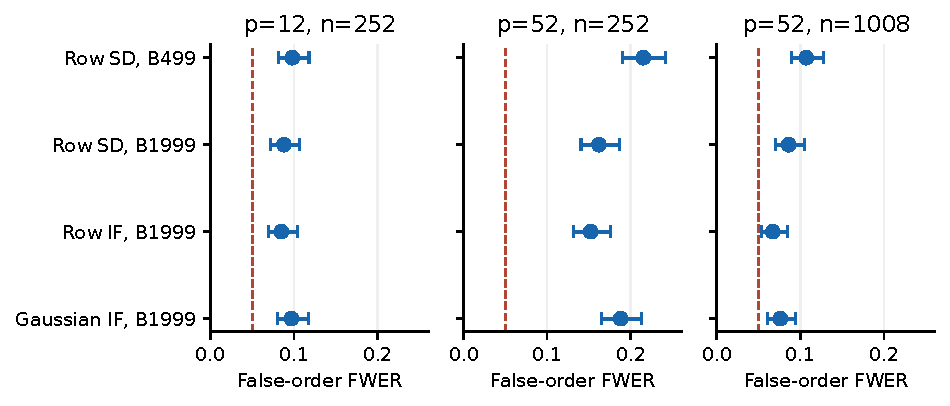
\includegraphics[width=\textwidth]{Fig_audit.pdf}
\caption{False-order FWER in the paired IID audit. Horizontal intervals are individual Wilson Monte Carlo intervals; the vertical line marks 0.05.}\label{fig:audit}\end{figure}



\section{Polish equity sensitivity study}\label{sec:gpw}
Polish stock correlation trees motivate the financial setting \citep{galazka2011}. A frozen historical assembly combines publicly available Bankier price histories, WIG observations and archived GPW index portfolios.\ifanonymous\else\ The input provenance and derived results are archived with immutable version identifiers \citep{previouscode}.\fi\ The base panel contains 231 origins from 2007--2025, each with 252 daily returns and 41--60 eligible stocks. Complete-history, positive-volume and nonzero-return checks are retained. Vendor prices are not certified dividend-inclusive total returns, extraordinary membership changes are not fully reconciled, and missing historical series prevent a complete licensed-market reconstruction.

Three representations---raw returns, cross-sectional demeaning and WIG residualization---use the same 999 circular block-bootstrap draws with block length ten, motivated by dependent resampling \citep{kunsch1989}, giving 693 base analyses. A fixed annual grid adds 466 analyses with nested liquid-stock groups, 252/504/1008-session lookbacks and block-length checks. These target Pearson trees and serially dependent returns. Their interpretation is sensitivity and temporal stability, separate from the exact Kendall IID applications above. Weekly or monthly nonoverlapping returns would not by themselves establish IID sampling.

Across matched stock groups, increasing the lookback from 252 to 1008 sessions reduces mean degree width by 13.9\%, 14.1\% and 10.3\% for groups of 10, 20 and 40 stocks. All rank ranges remain $[1,p]$. All 81 exclusions from the planned primary grid and 51 unavailable primary forward configurations per representation are retained. Full panel results and forward summaries are given in Section~\ref{sec:complete-gpw}; the independent checks of 109,548 improving rational certificates are described in Section~\ref{sec:baseline-verification}. This case study identifies a resolution limitation; it does not validate nominal bootstrap coverage for financial time series.

\section{Complete Polish-market sensitivity summaries}\label{sec:complete-gpw}
\begin{table}[htbp]
\caption{All 231 windows per representation. Widths are averages of the within-window mean degree width. Full ranks is the mean fraction of vertices with interval $[1,p]$. Hubs counts certified unique hubs over all windows. These are nominal bootstrap diagnostics.}\label{tab:gpw}
\centering\small
\begin{tabular}{lrrrr}
\toprule
Representation & Minor width & Path-LP width & Full ranks & Hubs \\
\midrule
Raw & 49.89 & 45.99 & 1.00 & 0 \\
Demeaned & 49.90 & 46.51 & 1.00 & 0 \\
WIG residual & 49.91 & 47.63 & 1.00 & 0 \\
\bottomrule
\end{tabular}
\end{table}
The refined projection reduces the raw-network mean degree width from 49.89 to 45.99, a 7.8\% reduction relative to the minor. It does not resolve hub ranks: all 35,979 reported vertex--window--representation rank intervals remain $[1,p]$. No unique hub and no top-decile membership is certified. There are 85,129 saved rational certificates for improved degree or anchor-contrast endpoints. These improvements demonstrate a stricter feasible-set projection, but not an informative financial hub ranking.

The complete panel leaves financial hub ranks unresolved under the stated Pearson calibrations and outer projections. The archived 24-cell diagnostic and paired IID audit document calibration limitations; these market ranges are interpreted as sensitivity outputs.

\subsection{Longer windows, nested liquid universes and forward diagnostics}\label{sec:extended}
The full-panel result motivates a sensitivity analysis that separates sample length from changing stock composition. Before computing the extended outcomes, we fixed the last recorded origin in every represented calendar year, giving 19 annual origins. The complete retrospective sensitivity grid and its unavailable cases are reported. At each origin, we use the longest calendar-available lookback from 504 and 1008 sessions to screen the original eligible list. Eligibility requires complete past returns, supplied prices and volumes, positive volume on at least 90\% of sessions, at most 15\% zero returns, and positive variance. Within this eligible set we rank stocks by median supplied closing price times volume, breaking ties by ISIN. This is an available-data liquidity proxy, not a certified corporate-action-adjusted traded-value measure.

We take nested groups of 10, 20 and 40 stocks. Their membership is kept fixed when comparing 252, 504 and 1008 sessions at the same origin. Changing group size changes the population tree target; a hub of a small liquid subnetwork need not be a hub of the full market. Demeaning is recomputed within each selected group, while factor residualization retains the same WIG series. All dated observations used for selection precede or coincide with the origin; future observations never enter selection. Vendor histories can incorporate later revisions, so this rule does not establish a fully point-in-time data source.

Of 513 planned origin--lookback--group--representation combinations, 81 cannot be evaluated because of insufficient calendar history or too few eligible stocks. We retain the full exclusion list. The remaining 432 primary analyses use block length ten and 999 common-row resamples per origin and lookback, across all three representations. A further 34 raw-network analyses examine block lengths five and twenty at $p=20,n=1008$, for all 17 available origins. These are nominal, per-configuration bootstrap projections. We do not claim simultaneous coverage over the grid or valid 95\% coverage for dependent returns.

\begin{table}[htbp]
\caption{Raw-network comparison on identical stocks and matched origins. The 1008-session availability criterion leaves 17 origins for groups of 10 and 20, and ten for groups of 40. Widths and forced-edge counts are within-group origin averages. Full ranks is the fraction of vertex ranges remaining $[1,p]$.}\label{tab:extended}
\centering\small
\begin{tabular}{rrrrrr}
\toprule
$p$ & Origins & $n$ & Degree width & Forced edges & Full ranks \\
\midrule
10 & 17 & 252 & 6.71 & 0.47 & 1.00 \\
10 & 17 & 504 & 6.18 & 0.59 & 1.00 \\
10 & 17 & 1008 & 5.78 & 1.00 & 1.00 \\
20 & 17 & 252 & 15.04 & 0.47 & 1.00 \\
20 & 17 & 504 & 14.14 & 0.65 & 1.00 \\
20 & 17 & 1008 & 12.92 & 1.35 & 1.00 \\
40 & 10 & 252 & 32.82 & 0.00 & 1.00 \\
40 & 10 & 504 & 31.03 & 0.20 & 1.00 \\
40 & 10 & 1008 & 29.45 & 0.80 & 1.00 \\
\bottomrule
\end{tabular}
\end{table}
The matched-origin mean degree width decreases by 13.9\%, 14.1\% and 10.3\% when moving from 252 to 1008 observations for groups of 10, 20 and 40 respectively. More edges are forced under the nominal order region, but none of the 432 primary or 34 block-sensitivity configurations yields a non-full vertex rank interval or a certified unique hub. The negative ranking result therefore survives a fourfold lookback extension, liquidity-based dimension reduction, and the stated block checks. This describes resolution for the stated procedures and targets.

\begin{table}[htbp]
\caption{Block-length sensitivity for the same 17 raw-network origins, $p=20,n=1008$. Resampling seeds differ between block lengths.}\label{tab:blocks}
\centering\small
\begin{tabular}{rrrrr}
\toprule
Block length & Origins & Degree width & Forced edges & Full ranks \\
\midrule
5 & 17 & 12.94 & 1.24 & 1.00 \\
10 & 17 & 12.92 & 1.35 & 1.00 \\
20 & 17 & 12.93 & 1.29 & 1.00 \\
\bottomrule
\end{tabular}
\end{table}
For a forward diagnostic, we hold the training stock group fixed and estimate a new tree using the next 252 sessions. The diagnostic is available only when every selected stock and the factor have complete future returns. We neither impute unavailable histories nor drop a future-missing stock from the selected group. There are 93 complete primary configurations per representation, out of 144; the remaining 51 have incomplete future histories or insufficient follow-up. Overlapping lookbacks and nested groups mean these are not 93 independent samples. Forward summaries are conditional on future-history availability and may be affected by attrition; no reweighting corrects that selection. We compute the fraction of transitive training order statements whose direction agrees with the future correlation estimates, and whether the training anchor remains tied for largest future degree. These are descriptive temporal-stability measures, not population coverage tests or portfolio-performance results.

\begin{table}[htbp]
\caption{Forward diagnostics over the next 252 sessions. Order agreement averages the within-configuration fractions, giving each configuration equal weight. Anchor still top includes ties and does not establish a unique hub.}\label{tab:forward}
\centering\small
\begin{tabular}{lrrr}
\toprule
Representation & Configurations & Order agreement & Anchor still top \\
\midrule
Raw & 93 & 95.7\% & 35/93 \\
Demeaned & 93 & 95.2\% & 19/93 \\
WIG residual & 93 & 93.9\% & 19/93 \\
\bottomrule
\end{tabular}
\end{table}
Estimated edge-order directions persist much more frequently than the identity of the estimated highest-degree vertex. This comparison involves different functionals: preservation of many inequalities is not equivalent to preservation of a hub, and a high fraction of correct directions need not mean that every direction is preserved jointly. Because the population can change over time, the forward sample is not a known-truth coverage benchmark. The calibration failures in Section~\ref{sec:simulation} remain unresolved.

As an illustration, the earliest complete raw-network configuration with anchor bootstrap frequency at least 0.9 and loss of top position in the future sample is the 2008 annual origin, $p=10,n=504$. The anchor is PKOBP; it is tied for highest degree in 91.2\% of bootstrap trees, while its nominal degree range is [1, 9] and rank range is [1, 10]. Its future estimated rank range is [3, 10], despite 100.0\% directional agreement for the certified training orders. The illustration is selected retrospectively by the stated rule; all configurations are reported, and it is not additional confirmatory evidence.

\begin{figure}[htbp]\centering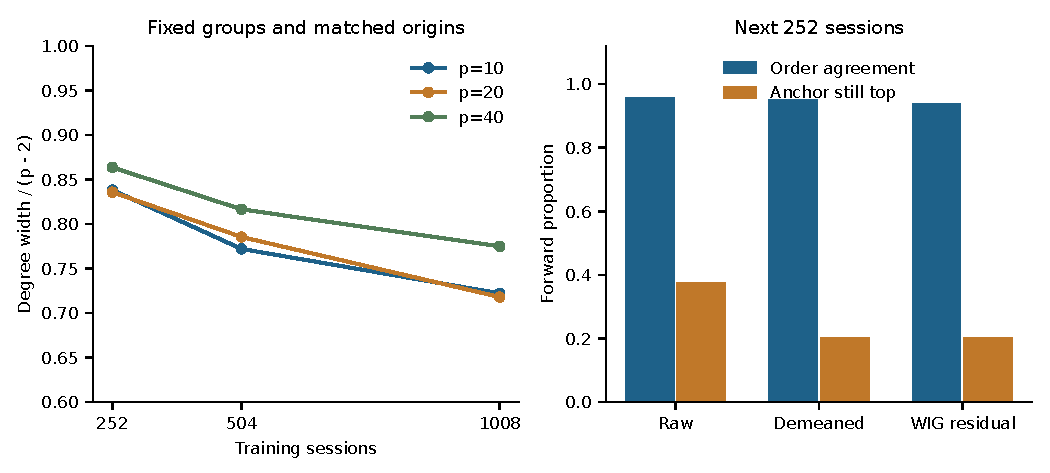
\includegraphics[width=\textwidth]{Fig_empirical.pdf}\caption{Extended empirical diagnostics. Left: mean raw-network degree width divided by $p-2$, on the matched origins and fixed stock groups in Table~\ref{tab:extended}. Right: forward edge-order agreement and retention of the training anchor among the highest-degree vertices, from Table~\ref{tab:forward}. Both panels are descriptive; neither supplies a validated confidence level for GPW returns.}\label{fig:empirical}\end{figure}
Independent verification reconstructs the selection rule for all 50 origin--group universes, checks five source-input hashes and all 9,710 additional vertex records, recomputes the 303 available forward analyses including block sensitivities, and validates all 24,419 improving rational LP certificates. Every check passes. Longer financial windows increase sample size while raising the possibility of regime changes, so their improved degree resolution must be interpreted alongside that stationarity limitation.

\section{Questionnaire split sensitivity}\label{sec:split-stability}

This post-application descriptive check retains all 100 additional random training splits and all 15 split-based variants. The dataset, training fraction, nominal level and 64 matchings are unchanged. Each split regenerates its associated matching randomization. The original full-sample E64 result is a fixed reference, not an E64 analysis restricted to each verification subset. No seed is selected to replace the reported application and no conclusions are pooled. The original internal protocol and application results entered the public archive together; there was no external preregistration. Consequently, this analysis measures descriptive sensitivity rather than prospectively registered validation.

A guaranteed shared member satisfies the degree-bound criterion in the main paper. At least two guaranteed members exclude a unique hub. Dominance of E64 means that all degree and rank intervals are subsets of the corresponding E64 intervals and every E64 guaranteed hub member is retained. Merely matching its number of fixed degrees is insufficient. All frequencies have denominator 100; they measure randomization stability conditional on the observed dataset, not population coverage probabilities.

\begin{table}[htbp]\centering\small\caption{All split variants under the common minor and conservation projection. Entries are counts out of 100 except the median. Three means joint membership of Q1, Q3 and Q10. No unique means unique-hub exclusion. Dominates uses the complete E64 comparison defined above.}\label{tab:split-methods}

\begin{tabular}{lrrrrr}\toprule Method & Median fixed & Three & No unique & $\ge6$ fixed & Dominates\\\midrule

FS-A64 & 5 & 7 & 7 & 49 & 48\\

FS-E64 & 5.5 & 10 & 10 & 50 & 49\\

FS-P & 1.5 & 4 & 5 & 11 & 10\\

FS-S64 & 1 & 0 & 0 & 0 & 0\\

FS-T64 & 6 & 16 & 16 & 62 & 61\\

H-A64 & 6 & 4 & 4 & 88 & 88\\

H-E64 & 6 & 6 & 6 & 94 & 94\\

H-P & 2 & 2 & 2 & 7 & 4\\

H-S64 & 4 & 0 & 0 & 0 & 0\\

H-T64 & 6 & 2 & 2 & 92 & 92\\

IUT-A64 & 0 & 0 & 0 & 0 & 0\\

IUT-E64 & 0 & 0 & 0 & 0 & 0\\

IUT-P & 0 & 2 & 2 & 2 & 2\\

IUT-S64 & 0 & 0 & 0 & 0 & 0\\

IUT-T64 & 0 & 0 & 0 & 0 & 0\\

\bottomrule\end{tabular}\end{table}

For FS-T64, the median number of fixed degrees is six, the interquartile range is four to six, and the range is one to eight. The reported split fixes eight degrees and is favourable. It is not representative of stability of the three-member conclusion, which is recovered in only 16 runs. FS-T64 retains all E64 bounds and memberships in 61 runs; it fixes at least six degrees in 62 runs. Exact enumeration is feasible for all 100 FS-T64 families (at most 495 candidate subsets). It gives the same shared-hub and unique-hub-exclusion decisions in every run, while degree endpoints agree with the minor in 76 runs and rank endpoints in 70 runs. Thus the observed hub instability is not an artefact of the minor relaxation.

\begin{table}[htbp]\centering\small\caption{FS-T64 guaranteed membership frequencies over 100 runs. Joint membership of Q1, Q3 and Q10 occurs in 16 runs.}\label{tab:split-items}\begin{tabular}{lrrrrrrrrrr}\toprule Item & Q1 & Q2 & Q3 & Q4 & Q5 & Q6 & Q7 & Q8 & Q9 & Q10\\\midrule

Count & 16 & 0 & 16 & 0 & 0 & 0 & 0 & 0 & 0 & 68\\\bottomrule\end{tabular}\end{table}

\begin{longtable}{rrrrrr}

\caption{Every FS-T64 split. Random seeds and all 15 variants are also archived as machine-readable records. Binary columns indicate joint three-member certification, unique-hub exclusion and dominance of E64.}\label{tab:all-splits}\\

\toprule Split & Seed & Fixed degrees & Three & No unique & Dominates\\\midrule\endfirsthead

\toprule Split & Seed & Fixed degrees & Three & No unique & Dominates\\\midrule\endhead

\midrule\multicolumn{6}{r}{Continued on next page}\\\endfoot\bottomrule\endlastfoot

1 & 2597299993 & 4 & 0 & 0 & 0\\

2 & 2066332529 & 3 & 0 & 0 & 0\\

3 & 2238539153 & 6 & 0 & 0 & 1\\

4 & 108058594 & 5 & 0 & 0 & 0\\

5 & 315714935 & 6 & 0 & 0 & 1\\

6 & 1158202976 & 3 & 0 & 0 & 0\\

7 & 253515632 & 6 & 0 & 0 & 1\\

8 & 1302646342 & 6 & 0 & 0 & 1\\

9 & 3098594182 & 6 & 0 & 0 & 1\\

10 & 1589487109 & 5 & 0 & 0 & 0\\

11 & 2686540733 & 4 & 0 & 0 & 0\\

12 & 4215396147 & 5 & 0 & 0 & 0\\

13 & 294088321 & 4 & 0 & 0 & 0\\

14 & 3961831916 & 8 & 1 & 1 & 1\\

15 & 1527441670 & 1 & 0 & 0 & 0\\

16 & 623582697 & 6 & 0 & 0 & 1\\

17 & 1005094014 & 8 & 1 & 1 & 1\\

18 & 45539246 & 2 & 0 & 0 & 0\\

19 & 1830072744 & 6 & 0 & 0 & 1\\

20 & 4293530424 & 4 & 0 & 0 & 0\\

21 & 1690465956 & 6 & 0 & 0 & 1\\

22 & 65281996 & 6 & 0 & 0 & 1\\

23 & 3372813861 & 2 & 0 & 0 & 0\\

24 & 3768342462 & 8 & 1 & 1 & 1\\

25 & 203936977 & 8 & 1 & 1 & 1\\

26 & 180148164 & 6 & 0 & 0 & 1\\

27 & 659924745 & 6 & 0 & 0 & 1\\

28 & 2450223545 & 3 & 0 & 0 & 0\\

29 & 2199508959 & 8 & 1 & 1 & 1\\

30 & 3605911653 & 8 & 1 & 1 & 1\\

31 & 1278973431 & 3 & 0 & 0 & 0\\

32 & 3786467762 & 6 & 0 & 0 & 1\\

33 & 3212858838 & 6 & 0 & 0 & 1\\

34 & 1320781665 & 6 & 0 & 0 & 1\\

35 & 3154359167 & 6 & 0 & 0 & 1\\

36 & 1493751066 & 6 & 0 & 0 & 1\\

37 & 190462844 & 5 & 0 & 0 & 0\\

38 & 3538048522 & 6 & 0 & 0 & 1\\

39 & 3876557283 & 4 & 0 & 0 & 0\\

40 & 739298930 & 6 & 0 & 0 & 1\\

41 & 3255724472 & 6 & 0 & 0 & 1\\

42 & 1771617184 & 6 & 0 & 0 & 1\\

43 & 3083054047 & 6 & 0 & 0 & 1\\

44 & 162745153 & 8 & 1 & 1 & 1\\

45 & 3764174810 & 5 & 0 & 0 & 0\\

46 & 846646590 & 6 & 0 & 0 & 1\\

47 & 236916371 & 8 & 1 & 1 & 1\\

48 & 251649469 & 6 & 0 & 0 & 1\\

49 & 2416785435 & 6 & 0 & 0 & 1\\

50 & 601269582 & 8 & 1 & 1 & 1\\

51 & 694590042 & 6 & 0 & 0 & 1\\

52 & 2375188160 & 6 & 0 & 0 & 1\\

53 & 811775620 & 2 & 0 & 0 & 0\\

54 & 864718370 & 6 & 0 & 0 & 1\\

55 & 206384097 & 6 & 0 & 0 & 0\\

56 & 4257859691 & 6 & 0 & 0 & 1\\

57 & 287556693 & 6 & 0 & 0 & 1\\

58 & 3008046515 & 1 & 0 & 0 & 0\\

59 & 1273941298 & 8 & 1 & 1 & 1\\

60 & 2073878958 & 8 & 1 & 1 & 1\\

61 & 1660843960 & 6 & 0 & 0 & 1\\

62 & 3838832839 & 4 & 0 & 0 & 0\\

63 & 1299057954 & 3 & 0 & 0 & 0\\

64 & 575788243 & 6 & 0 & 0 & 1\\

65 & 831898435 & 2 & 0 & 0 & 0\\

66 & 3133827474 & 5 & 0 & 0 & 0\\

67 & 1901459113 & 6 & 0 & 0 & 1\\

68 & 4219504914 & 4 & 0 & 0 & 0\\

69 & 2081332392 & 2 & 0 & 0 & 0\\

70 & 1350502935 & 6 & 0 & 0 & 1\\

71 & 4178251367 & 6 & 0 & 0 & 1\\

72 & 2613697323 & 1 & 0 & 0 & 0\\

73 & 3288342582 & 2 & 0 & 0 & 0\\

74 & 4244313923 & 4 & 0 & 0 & 0\\

75 & 3802243133 & 8 & 1 & 1 & 1\\

76 & 263771850 & 5 & 0 & 0 & 0\\

77 & 1733575506 & 4 & 0 & 0 & 0\\

78 & 442334869 & 6 & 0 & 0 & 1\\

79 & 1950752074 & 6 & 0 & 0 & 1\\

80 & 2730877703 & 4 & 0 & 0 & 0\\

81 & 751278161 & 5 & 0 & 0 & 0\\

82 & 1524820730 & 6 & 0 & 0 & 1\\

83 & 4264146325 & 6 & 0 & 0 & 1\\

84 & 198038047 & 2 & 0 & 0 & 0\\

85 & 1524174271 & 6 & 0 & 0 & 1\\

86 & 2352447263 & 8 & 1 & 1 & 1\\

87 & 379334832 & 2 & 0 & 0 & 0\\

88 & 548276364 & 6 & 0 & 0 & 1\\

89 & 1632308413 & 3 & 0 & 0 & 0\\

90 & 3343177532 & 6 & 0 & 0 & 1\\

91 & 339188587 & 8 & 1 & 1 & 1\\

92 & 3821830014 & 6 & 0 & 0 & 1\\

93 & 2804609772 & 2 & 0 & 0 & 0\\

94 & 234850423 & 6 & 0 & 0 & 1\\

95 & 2490516670 & 2 & 0 & 0 & 0\\

96 & 162639027 & 8 & 1 & 1 & 1\\

97 & 1842484868 & 6 & 0 & 0 & 1\\

98 & 3544619934 & 1 & 0 & 0 & 0\\

99 & 1099956211 & 6 & 0 & 0 & 1\\

100 & 275712381 & 8 & 1 & 1 & 1\\

\end{longtable}

Independent checks recompute the summary counts from all saved records, verify the accepted trees and their degree ranges, and replay split indices 1, 50 and 100 from the original data. A separate Boolean-closure implementation reproduces the complete compatible-tree sets for these replays. The individual finite-sample guarantee remains a statement about one fixed procedure; these tables do not carry joint 95\% coverage across methods or reruns.

\bibliographystyle{plainnat}\bibliography{references,new_references}
\end{document}
